%% =====================================================================
%%  Aieva - project documentation (two pages)
%%  Compile with:  pdflatex Aieva_Project_Documentation.tex
%%                 (or: tectonic Aieva_Project_Documentation.tex)
%% =====================================================================
\documentclass[10pt,a4paper]{article}

\usepackage[T1]{fontenc}
\usepackage[utf8]{inputenc}
\usepackage{lmodern}
\usepackage[a4paper,top=1.6cm,bottom=1.6cm,left=1.7cm,right=1.7cm]{geometry}
\usepackage{xcolor}
\usepackage{booktabs}
\usepackage{array}
\usepackage{enumitem}
\usepackage{tikz}
\usepackage{titlesec}
\usepackage[hidelinks]{hyperref}
\usetikzlibrary{arrows.meta,positioning,fit,backgrounds}

\definecolor{aievaBlue}{HTML}{1F4E79}
\definecolor{aievaGreen}{HTML}{2E7D32}
\definecolor{aievaGrey}{HTML}{F2F4F7}

\titleformat{\section}{\normalfont\large\bfseries\color{aievaBlue}}{\thesection.}{0.6em}{}
\titleformat{\subsection}{\normalfont\normalsize\bfseries\color{aievaBlue}}{\thesubsection.}{0.5em}{}
\titlespacing{\section}{0pt}{6pt}{3pt}
\titlespacing{\subsection}{0pt}{4pt}{2pt}

\setlength{\parindent}{0pt}
\setlength{\parskip}{3pt}
\setlist[itemize]{leftmargin=1.2em,itemsep=0.5pt,topsep=2pt}
\setlist[enumerate]{leftmargin=1.4em,itemsep=0.5pt,topsep=2pt}

\begin{document}

% ----------------------------------------------------------------- title
\begin{center}
  {\LARGE\bfseries\color{aievaBlue} Aieva}\\[2pt]
  {\large Screen-aware AI educational visualization assistant (Math edition)}\\[3pt]
  {\small Windows desktop app (Kivy) + local fog server (FastAPI) in front of Gemini}
\end{center}

\hrule\vspace{6pt}

% ------------------------------------------------------------------ what
\section*{1. What the project is}

Aieva is a helper for the \emph{interactive board} of a classroom. The teacher
selects a region of the board with the mouse or the finger, Aieva reads the
writing with \textbf{Gemini}, understands what it is (an equation, a graph, a
table of numbers, a word problem), computes the answer with \textbf{SymPy} and
shows it in a small window on the board: the steps of the solution, the graph,
the chart, the integral. Nothing has to be typed, nothing has to be copied, and
no other tool has to be opened.

The project is a real working application, not a prototype: the maths is
checked by SymPy, the Windows parts are scripted, and the whole thing is
covered by an automated test suite (\textbf{783 passed, 3 skipped}).

% ------------------------------------------------------------ architecture
\section*{2. Architecture and workflow}

Aieva is split into a \emph{headless core} (pure maths, no screen), a
\emph{Kivy user interface} (the app, the floating control, the charts) and a
\emph{fog server} (the only part that talks to Google). This split is what
makes the project testable: 90\,\% of the code never touches a window.

\begin{center}
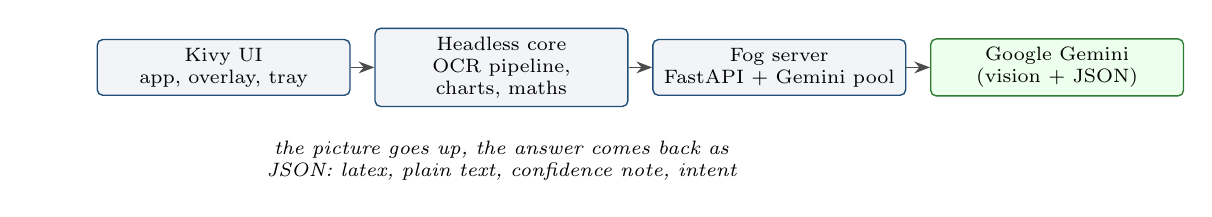
\begin{tikzpicture}[
  font=\scriptsize,
  node distance=3mm,
  box/.style={draw=aievaBlue, rounded corners=2pt, fill=aievaGrey,
              text width=30mm, align=center, inner sep=3pt, line width=0.5pt},
  cloud/.style={draw=aievaGreen, rounded corners=2pt, fill=green!7,
                text width=30mm, align=center, inner sep=3pt, line width=0.5pt},
  arrow/.style={-{Stealth[length=2mm]}, line width=0.5pt, draw=black!70}
]
\node[box] (ui) {Kivy UI\\app, overlay, tray};
\node[box, right=of ui] (core) {Headless core\\OCR pipeline, charts, maths};
\node[box, right=of core] (srv) {Fog server\\FastAPI + Gemini pool};
\node[cloud, right=of srv] (gem) {Google Gemini\\(vision + JSON)};
\draw[arrow] (ui) -- (core);
\draw[arrow] (core) -- (srv);
\draw[arrow] (srv) -- (gem);
\node[font=\scriptsize\itshape, below=3mm of core, text width=118mm, align=center]
  {the picture goes up, the answer comes back as JSON: latex, plain text, confidence note, intent};
\end{tikzpicture}
\end{center}

\textbf{The workflow of one reading.}

\begin{enumerate}
\item The teacher drags the compact control on the \textbf{left edge} of the
      board and picks the region to read (or presses \emph{Scan}).
\item The region is captured and sent to the fog server.
\item The server sends the picture to Gemini with a strict JSON prompt and
      gets back: the LaTeX, the plain text, a confidence note, the kind of the
      content and the \textbf{intent} (explain, solve, plot, integrate, chart,
      word problem).
\item The intent routes the answer: SymPy solves and simplifies, Matplotlib
      draws the 2D/3D graph, the chart renderer draws the table, the templates
      build the step-by-step explanation.
\item The result is published to the service and shown in the popup of the
      overlay (or in the full app of the teacher).
\end{enumerate}

% --------------------------------------------------------------- features
\section*{3. Main features}

\begin{itemize}
\item \textbf{Board OCR with Gemini.} The picture of the board becomes
      structured JSON (LaTeX + plain text + confidence note). No Tesseract, no
      manual typing.
\item \textbf{Intent routing.} One model, many answers: the same prompt asks
      for the intent, so a graph and an integral are never sent to the wrong
      place.
\item \textbf{Maths core (SymPy).} Solving, simplification, derivatives,
      definite and indefinite integrals, limits, series, linear algebra
      (matrices, systems, complex numbers) and statistics --- every answer is
      verified symbolically, never by string matching.
\item \textbf{2D and 3D graphs.} A real Matplotlib canvas inside Kivy:
      rotation, zoom and parameter sliders for the 3D surfaces.
\item \textbf{Charts.} Bar, line and pie charts are rendered by
      \texttt{aieva/core/charts.py}. The renderer is \emph{subject-agnostic}:
      the maths uses it, and so can physics (motion graphs), chemistry
      (concentration curves) and biology (population charts).
\item \textbf{Word problems.} The text is split into variables, equations and
      unknowns, then solved with sliders for the unknown parameters.
\item \textbf{Documents.} PDF, Word and PowerPoint are read and turned into
      pictures or text for the same pipeline.
\item \textbf{Background service.} Aieva watches the board in the background,
      shows a compact control on the left edge of the screen and puts the
      answer where the teacher is looking.
\item \textbf{Automatic start.} The service registers itself in the Windows
      task scheduler: \texttt{ONSTART} first, \texttt{ONLOGON} without
      administrator rights, and the startup folder as the last fallback.
\item \textbf{Pool of Gemini keys.} Several keys live in the \texttt{.env};
      a key whose quota is gone is skipped at once and the next one answers.
      The fallback stays \emph{inside} Gemini --- the OCR needs a model that
      reads a picture.
\item \textbf{Doctor.} One command checks Python, the packages, the
      \texttt{.env}, the server, the OCR, the capture, the autostart and the
      service, and says exactly what to fix.
\item \textbf{Mock mode.} With \texttt{AIEVA\_MOCK\_LLM=true} the whole
      application runs without a key and without the network --- the mode the
      tests use.
\end{itemize}

% -------------------------------------------------------------- install
\section*{4. Installation and use}

\begin{enumerate}
\item \textbf{Install.} \texttt{powershell -ExecutionPolicy Bypass -File
      scripts\textbackslash setup.ps1} creates the virtual environment
      (\texttt{.venv}), installs \texttt{requirements.txt} +
      \texttt{requirements-server.txt} and writes the \texttt{.env}.
\item \textbf{The key.} In \texttt{.env}:
      \texttt{GEMINI\_API\_KEY=...} and, if there is more quota,
      \texttt{GEMINI\_API\_KEYS=key2,key3} (comma separated). The
      \texttt{GEMINI\_MODEL} chooses the Flash model.
\item \textbf{The server.} \texttt{.\textbackslash scripts\textbackslash
      run\_server.ps1} starts the fog server on
      \texttt{http://127.0.0.1:8000}; it must run before the board is read.
\item \textbf{The start.} \texttt{.\textbackslash
      scripts\textbackslash install\_autostart.ps1} registers the task (run
      PowerShell as administrator for the boot variant).
\item \textbf{The check.} \texttt{.venv\textbackslash Scripts\textbackslash
      python.exe -m aieva.core.doctor}.
\item \textbf{Use.} \texttt{python -m aieva.ui.app} for the full application
      or \texttt{python -m aieva.core.service run --overlay --tray} for the
      background service with the floating control and the tray icon.
\end{enumerate}

\section*{5. Testing}

\begin{center}
\begin{tabular}{@{}ll@{}}
\toprule
\textbf{Command} & \textbf{What it does} \\
\midrule
\texttt{python -m pytest tests -q} & the whole suite: 783 passed, 3 skipped \\
\texttt{python -m ruff check .} & the linter (no error allowed) \\
\texttt{python -m black --check .} & the formatter \\
\texttt{python -m aieva.core.doctor} & is this PC ready for the board? \\
\bottomrule
\end{tabular}
\end{center}

The suite is split in unit tests (the maths, the charts, the parsing, the
configuration, the pool of the keys) and integration tests (the OCR pipeline,
the server, the Kivy screens, the tray, the scripts of Windows). The three
skipped tests need a real Gemini key.

% --------------------------------------------------------------- limits
\section*{6. Limitations and future work}

\begin{itemize}
\item \textbf{No offline version.} Gemini reads the board, so a network and a
      key are needed. The mock mode is for the development, not for a lesson.
\item \textbf{No engine reads every handwriting perfectly.} Glare, an
      occlusion or an unusual notation can be misread; that is why every
      answer is verified by SymPy and the confidence note of Gemini is shown
      next to it.
\item \textbf{The Windows parts need a real board PC.} The task of the task
      scheduler, the tray icon, the capture of the screen, the place of the
      windows and the PowerShell scripts are written and unit-tested, but the
      autostart, the tray and the capture still have to be tried on the real
      hardware.
\item \textbf{The key pool is a fallback, not a load balancer.} The keys are
      used one after the other; parallel requests do not spread over the pool.
\item \textbf{Next steps.} The chat/canvas mode (\texttt{AIEVA\_BOARD\_MODE=1},
      Aieva becomes the board and needs no screen capture), the Android port
      (parked in \texttt{APK-LATER}) and a teachers' log of the answers.
\end{itemize}

\vfill
\hrule\vspace{3pt}
{\footnotesize\itshape Aieva --- screen-aware AI educational visualization
assistant (Math edition). MIT licence. The full guide lives in
\texttt{shuvojit.md}; the code in the repository.}

\end{document}
